%%%%%%%%%%%%%%%%%%%%%%%%%%%%%%%%%%%%%%%%%
% Beamer Presentation
% LaTeX Template
% Version 1.0 (10/11/12)
%
% This template has been downloaded from:
% http://www.LaTeXTemplates.com
%
% License:
% CC BY-NC-SA 3.0 (http://creativecommons.org/licenses/by-nc-sa/3.0/)
%
%%%%%%%%%%%%%%%%%%%%%%%%%%%%%%%%%%%%%%%%%

%----------------------------------------------------------------------------------------
%	PACKAGES AND THEMES
%----------------------------------------------------------------------------------------

\documentclass{beamer}

\mode<presentation> {

% The Beamer class comes with a number of default slide themes
% which change the colors and layouts of slides. Below this is a list
% of all the themes, uncomment each in turn to see what they look like.

%\usetheme{default}
%\usetheme{AnnArbor}
%\usetheme{Antibes}
%\usetheme{Bergen}
%\usetheme{Berkeley}
%\usetheme{Berlin}
%\usetheme{Boadilla}
%\usetheme{CambridgeUS}
%\usetheme{Copenhagen}
%\usetheme{Darmstadt}
%\usetheme{Dresden}
%\usetheme{Frankfurt}
%\usetheme{Goettingen}
%\usetheme{Hannover}
%\usetheme{Ilmenau}
%\usetheme{JuanLesPins}
%\usetheme{Luebeck}
\usetheme{Madrid}
%\usetheme{Malmoe}
%\usetheme{Marburg}
%\usetheme{Montpellier}
%\usetheme{PaloAlto}
%\usetheme{Pittsburgh}
%\usetheme{Rochester}
%\usetheme{Singapore}
%\usetheme{Szeged}
%\usetheme{Warsaw}

% As well as themes, the Beamer class has a number of color themes
% for any slide theme. Uncomment each of these in turn to see how it
% changes the colors of your current slide theme.

%\usecolortheme{albatross}
%\usecolortheme{beaver}
%\usecolortheme{beetle}
%\usecolortheme{crane}
%\usecolortheme{dolphin}
%\usecolortheme{dove}
%\usecolortheme{fly}
%\usecolortheme{lily}
%\usecolortheme{orchid}
%\usecolortheme{rose}
%\usecolortheme{seagull}
%\usecolortheme{seahorse}
%\usecolortheme{whale}
%\usecolortheme{wolverine}

%\setbeamertemplate{footline} % To remove the footer line in all slides uncomment this line
%\setbeamertemplate{footline}[page number] % To replace the footer line in all slides with a simple slide count uncomment this line

%\setbeamertemplate{navigation symbols}{} % To remove the navigation symbols from the bottom of all slides uncomment this line
}
\usepackage{caption}% http://ctan.org/pkg/caption
\usepackage{graphicx} % Allows including images
\usepackage{booktabs} % Allows the use of \toprule, \midrule and \bottomrule in tables
\captionsetup[figure]{labelformat=empty}%
%----------------------------------------------------------------------------------------
%	TITLE PAGE
%----------------------------------------------------------------------------------------

\title[Autononous Parking Space Analysis]{Autonomous Parking Space Analysis} % The short title appears at the bottom of every slide, the full title is only on the title page

\author{Julien Nyambal} % Your name
\institute[WITS] % Your institution as it will appear on the bottom of every slide, may be shorthand to save space
{
University of the Witwatersrand, Johannesburg \\ % Your institution for the title page
\medskip
%\textit{john@smith.com} % Your email address
}

\date[\today]{} % Date, can be changed to a custom date

\begin{document}

\begin{frame}
\titlepage % Print the title page as the first slide
\end{frame}

\begin{frame}
\frametitle{Overview} % Table of contents slide, comment this block out to remove it
\tableofcontents % Throughout your presentation, if you choose to use \section{} and \subsection{} commands, these will automatically be printed on this slide as an overview of your presentation
\end{frame}

%----------------------------------------------------------------------------------------
%	PRESENTATION SLIDES
%----------------------------------------------------------------------------------------

%------------------------------------------------
\section{Introduction} % Sections can be created in order to organize your presentation into discrete blocks, all sections and subsections are automatically printed in the table of contents as an overview of the talk
%------------------------------------------------

\subsection{Description}

\begin{frame}
\frametitle{Description}

The project aims to automatically predict the availability of a parking spot given the feeds provided by a video camera monitoring the parking area. 

\end{frame}

%--------------------------------------------------------
\subsection{Motivation}

\begin{frame}
\frametitle{Motivation}

\begin{block}{\textbf{Hunting for parking brings no joy for students}\cite{wits}}
``...Students at Wits are struggling to find available parking spaces on campuses since...''\\ 
``...student X said that finding parking is the biggest issue she faces at Wits.''
\\[5pt]
\rightline{{\rm --- Aarti Bhana, Wits Vuvuzela}}
\end{block}
\end{frame}

%------------------------------------------------
\subsection{Problems}
\begin{frame}
\frametitle{Problems}
Various factors can explain the parking space problems mostly in urban areas:

\begin{itemize}
\item Urban planning not following the quick growth of population dynamics
\item Drivers not aware of available space due to lack of knowledge of the area or anything obstructing it from the driver 
\item Bad management of the parking area
\end{itemize}
\end{frame}

%------------------------------------------------
\subsection{Aims}
\begin{frame}
\frametitle{Aims}

This project aims to:

\begin{itemize}
\item Perform comparative study between existing solutions (SVM based algorithms) and CNN,
\item Use video cameras to allocate parking spaces to drivers
\item Apply computer vision techniques to infer the status of a space (Background subtraction, Hough transform ...),
\item Help the driver to locate a vacant spot using the dedicated web application,
\item Run a quantitative analysis of the results produced by the system to predict parking habits of drivers.
\end{itemize}

\end{frame}

%------------------------------------------------
\section{Background and related work}
%------------------------------------------------

\subsection{Sensors Based Detection}

\begin{frame}
\frametitle{Sensors Based Detection}

\begin{figure}[!htbp]
  \centering
  \begin{minipage}[b]{0.5\textwidth}
    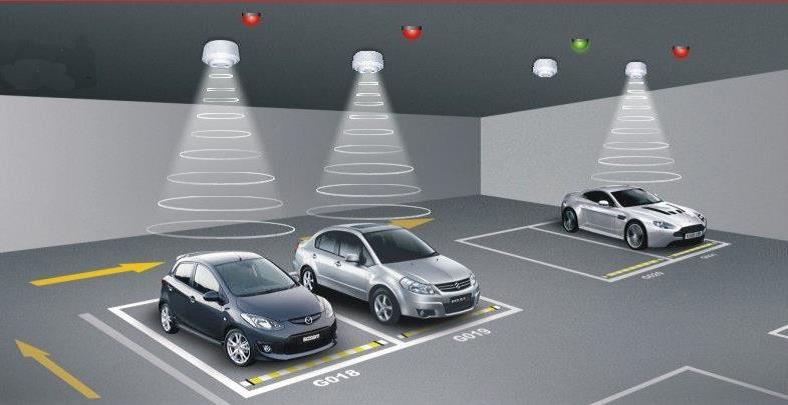
\includegraphics[width=\textwidth]{Pictures/overhead}
    \caption{Non-intrusive sensors, \cite{overhead}}
    \label{nonintru}
  \end{minipage}
  \hfill
  \begin{minipage}[b]{0.4\textwidth}
    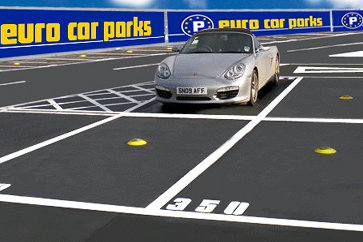
\includegraphics[width=\textwidth]{Pictures/sensor}
    \caption{Intrusive sensors, \cite{ground}}
    \label{intru}
  \end{minipage}
\end{figure}

\end{frame}

\begin{frame}
\frametitle{Sensors Based Detection}

Pros:
\begin{itemize}
	\item Very accurate,
	\item Since individually installed per spot, the system can return the available number of spots \cite{Lee2008},
	\item Almost no computation required
\end{itemize}

Cons:
\begin{itemize}
	\item Expensive in installation in terms of number of devices to place per spot,
	\item Expensive in maintenance.
\end{itemize}

\end{frame}
%------------------------------------------------

\subsection{Video Based Methods}

\begin{frame}
\frametitle{Traditional Image Processing}
\begin{enumerate}
\item Background subtraction to create a transience map of the parking area or to model the parking area given the previous positions of vehicles
\item 
\end{enumerate}
\end{frame}

\begin{frame}[allowframebreaks]
\frametitle{Background Subtraction}
\begin{block}{Definition}
The background subtraction is a technique used in computer vision and image processing for detecting the foreground from a set a images of the same scenario (video sequence of a non-moving camera) for various types of detection problems.
\begin{equation}
|frame_i - frame_{i-1}| > T_h 
\label{diff_frame}
\end{equation}
\end{block}
\vspace{5cm}
\begin{figure}[!htbp]
	\begin{minipage}[b]{0.48\textwidth}
		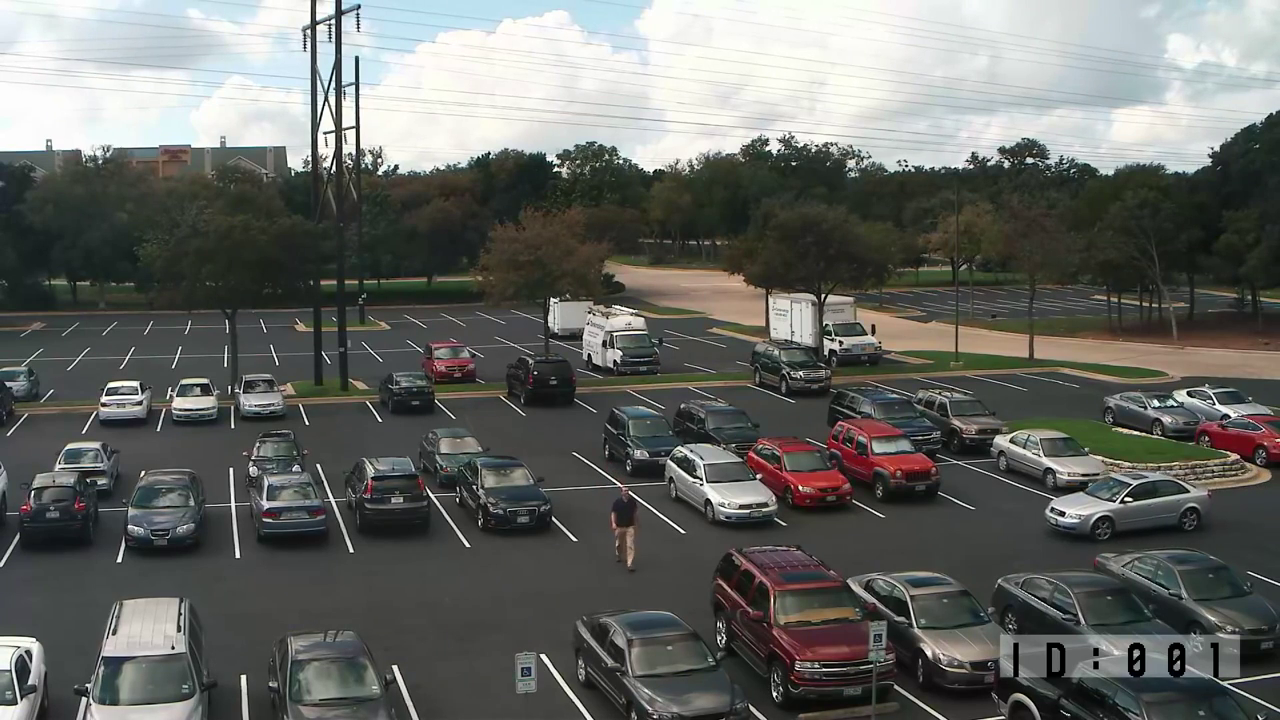
\includegraphics[width=\textwidth]{Pictures/fg308}
		\caption{Original image}
		\label{foreground}
	\end{minipage}
	\hfill
	\begin{minipage}[b]{0.48\textwidth}
		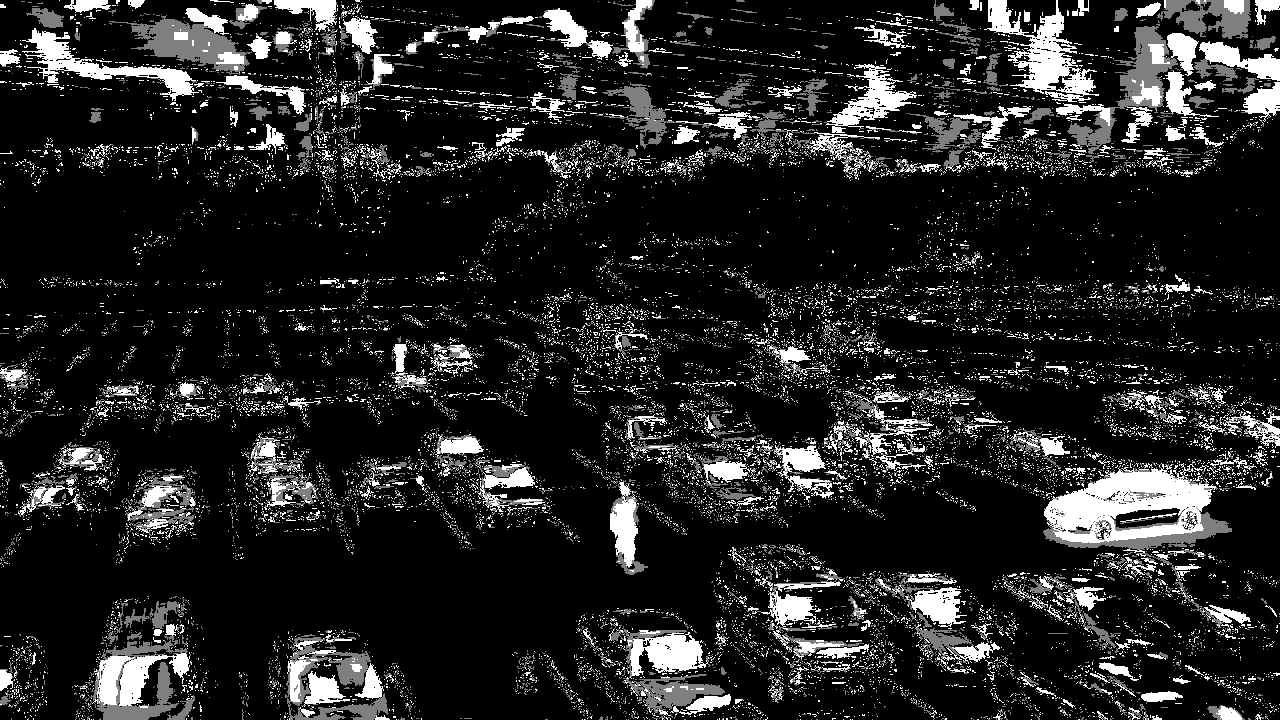
\includegraphics[width=\textwidth]{Pictures/bg308}
		\caption{Background subtracted image}
		\label{background}
	\end{minipage}
\end{figure}
\vspace{5cm}
Background subtraction to:
\begin{itemize}
	\item Create a transience map of the parking area or to model the parking area given the previous positions of vehicles \cite{Postigo}
	\begin{figure}
		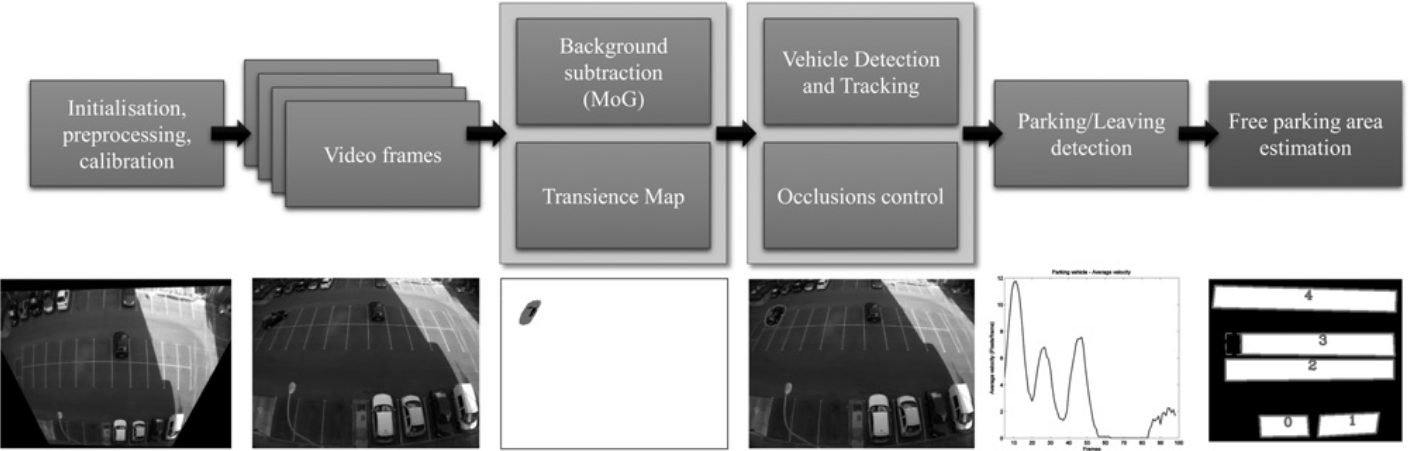
\includegraphics[width=300pt]{Pictures/transmap}
		\caption{Background subtraction method proposed by \cite{Postigo}}
	\end{figure}
	This method used the background subtraction and the Mixture of Gaussians to detect and track vehicles to infer the availability of remaining spots given a \textbf{threshold} on the transient value, 
	\item Use histograms of spatial features to map the spots of an unmanaged parking area but taking as object the group of pixels generated by vehicles, rejecting the non-vehicle objects by automatically adjusting the \textbf{threshold} \cite{Choeychuen}.
\end{itemize}


\end{frame}

\begin{frame}[allowframebreaks]
\frametitle{Support Vector Machines}
Definition:\\
Supervised machine learning technique that is based on a decision boundary to separate data into different subsets (classes). Support vectors are the coordinates of data point in the data space that are the closest to the boundary lines, hyperplanes.\\
Support Vector Machines(SVM) can be used for \textbf{classification} and \textbf{regression} problems. The classification has been mostly used for the parking space detection.

\begin{figure}[h!]
	%should be after intrinsic calibration
	\centering
	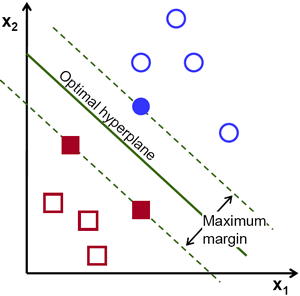
\includegraphics[width=0.4\textwidth]{Pictures/SVM}
	\caption{Support Vector Machines, OpenCVDocs}
\end{figure}

Support Vector Machines (SVM) have been widely used for the problem. Usually associated with Histograms of Oriented Gradients (HoG), Difference of Gaussians (DoG), color histograms, Local Binary Patterns...

\end{frame}

\begin{frame}
\frametitle{Deep Learning - Convolutional Neural Networks }

\begin{block}{Definition}

\begin{itemize}
\item Spervised branch of machine learning for pattern and object recognition,
\item CNN learn extracted features,
\item CNN are computationally expensive at the training phase especially when the dataset contains many classes with many objects to classify
\end{itemize}

\end{block}
\end{frame}

\begin{frame}
\frametitle{Deep Learning - Convolutional Neural Networks }

\begin{figure}[h!]
%should be after intrinsic calibration
    \centering
    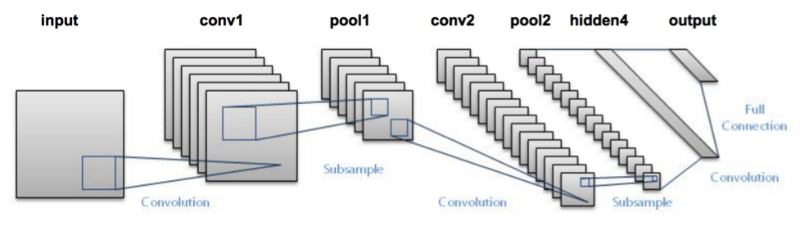
\includegraphics[width=0.9\textwidth]{Pictures/lenet_architecture}
    \caption{Lenet-5, \cite{Lecun98gradient-basedlearning}}
\end{figure}

\end{frame}


%----------------------------------------
\section{What's next}

\begin{frame}
\frametitle{Path to follow}
\begin{block}{Guidelines}
Our main objectives will be to:
\begin{itemize}
\item Compare the performance of the mainly used classifiers based on the literature review: CNN and SVM,
\item Collect data for the new experiments to do based on the classifier we will choose,
\item Design and implement an algorithm that will automatically withdraw the parking bays to feed them to the classifier (Hough transform for example) given the whole parking lot
\item Perform a qualitative analysis of the usage of the parking as a whole to predict the availability of the bays.

\end{itemize}

\end{block}
\end{frame}

%-----------------------------------------------

\begin{frame}
\Huge{\centerline{End}}
\end{frame}

%----------------------------------------------------------------------------------------

%------------------------------------------------
\section{References}
%------------------------------------------------
\begin{frame}[allowframebreaks]{References}%in case more than 1 slide needed
\footnotesize{
\bibliographystyle{ieeetr}
\bibliography{reference.bib}}
\end{frame}
\end{document}

\end{document}